\documentclass{beamer}

\usepackage{clrscode3e}
\usepackage{amsmath}
\usepackage{graphicx}
\usepackage{multicol}

\newcommand{\bi}{\begin{itemize}}
\newcommand{\ii}{\item}
\newcommand{\ei}{\end{itemize}}
\newcommand{\bn}{\begin{enumerate}}
\newcommand{\en}{\end{enumerate}}
\newcommand{\set}[1]{\ensuremath{\left\{#1\right\}}}
\newcommand{\pr}[1]{\ensuremath{\mbox{Pr}\left\{#1\right\}}}
\newcommand{\flr}[1]{\ensuremath{\left\lfloor#1\right\rfloor}}
\newcommand{\ceil}[1]{\ensuremath{\left\lceil#1\right\rceil}}

\newcommand{\sect}[1]{
\section{#1}
\begin{frame}[fragile]\frametitle{#1}
}



\title{Notes on Quicksort}
\author{Geoffrey Matthews}
\begin{document}
\begin{frame}
  \maketitle
\end{frame}

\sect{Quicksort}
\bi
\ii $\Theta(n^2)$ worst case.
\ii $\Theta(n\lg n)$ expected running time.
\ii Constants are small.
\ii Sorts in place.
\ei

\end{frame}

\sect{Quicksort: three step process}
\bi
\ii To sort $A[p..r]$:
\bi
\ii \textbf{Divide:} Partition  $A[p..r]$ into two (possibly empty)
subarrays\\ $A[p..q-1]$ and $A[q+1..r]$,\\ such that each element
in the first subarray is $\leq A[q]$\\ and $A[q] \leq$ each element in the
second subarray.
\ii \textbf{Conquer:} Sort the two subarrays by recursive calls.
\ii \textbf{Combine:} Nothing needs to be done.
\ei
\ei
  

\begin{codebox}
  \Procname{$\proc{Quicksort}(A,p,r)$}
  \li \If $p < r$ \Do
  \li $q\gets \proc{Partition}(A,p,r)$
  \li $\proc{Quicksort}(A,p,q-1)$
  \li $\proc{Quicksort}(A,q+1,r)$
\End
\end{codebox}

Initial call is \textsc{Quicksort$(A,1,n)$}

\end{frame}

\sect{Compare \textsc{Quicksort} and \textsc{Mergesort}}

  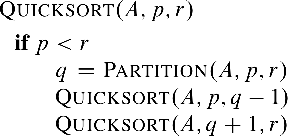
\includegraphics{Quicksort}
  \vfill
  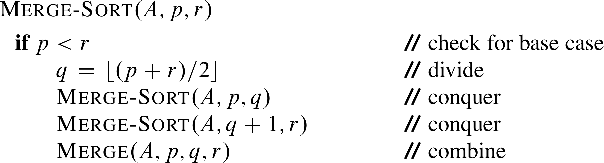
\includegraphics{Merge-Sort}


\end{frame}

\sect{Compare \textsc{Partition} and \textsc{Merge}}

  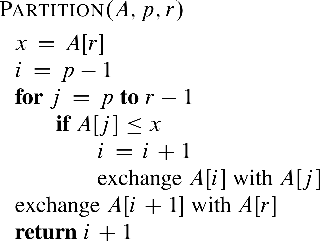
\includegraphics[scale=0.8]{Partition}
  \hfill
  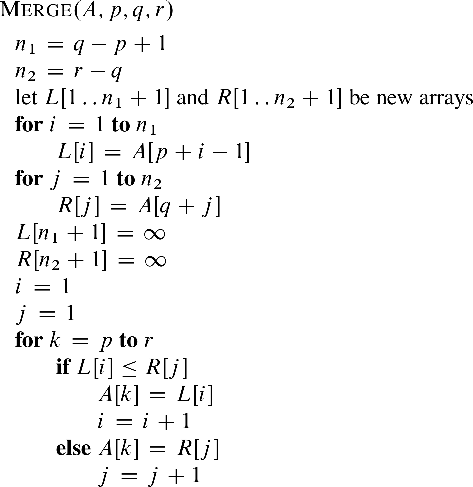
\includegraphics[scale=0.8]{Merge}


\end{frame}

%\begin{minipage}{4in}
%\begin{codebox}
%  \Procname{$\proc{Quicksort}(A,p,r)$}
%  \li \If $p < r$ \Do
%  \li $q\gets \proc{Partition}(A,p,r)$
%  \li $\proc{Quicksort}(A,p,q-1)$
%  \li $\proc{Quicksort}(A,q+1,r)$
%\End
%\end{codebox}
%\end{minipage}\hfill
%  \begin{minipage}{4in}
%\begin{codebox}
%  \Procname{$\proc{Mergesort}(A,p,r)$}
%  \li \If $p < r$ \Do
%  \li $q\gets \lfloor (p+r)/2 \rfloor$
%  \li $\proc{Mergesort}(A,p,q)$
%  \li $\proc{Mergesort}(A,q+1,r)$
%  \li $\proc{Merge}(A,p,q,r)$
%\End
%\end{codebox}
%  \end{minipage}
%  
%
%\newpage
%\begin{minipage}{5in}
%\begin{codebox}
%  \Procname{$\proc{Partition}(A,p,r)$}
%  \li $x \gets A[r]$
%  \li $i\gets p-1$
%  \li \For $j=p$ \To $r-1$ \Do
%  \li \If $A[j] \leq x$ \Do
%  \li $i \gets i+1$
%  \li exchange $A[i]$ with $A[j]$
%\End
%\End
%\li exchange $A[i+1]$ with $A[r]$
%\li \Return $i+1$
%\end{codebox}
%\end{minipage}

\sect{Partition}

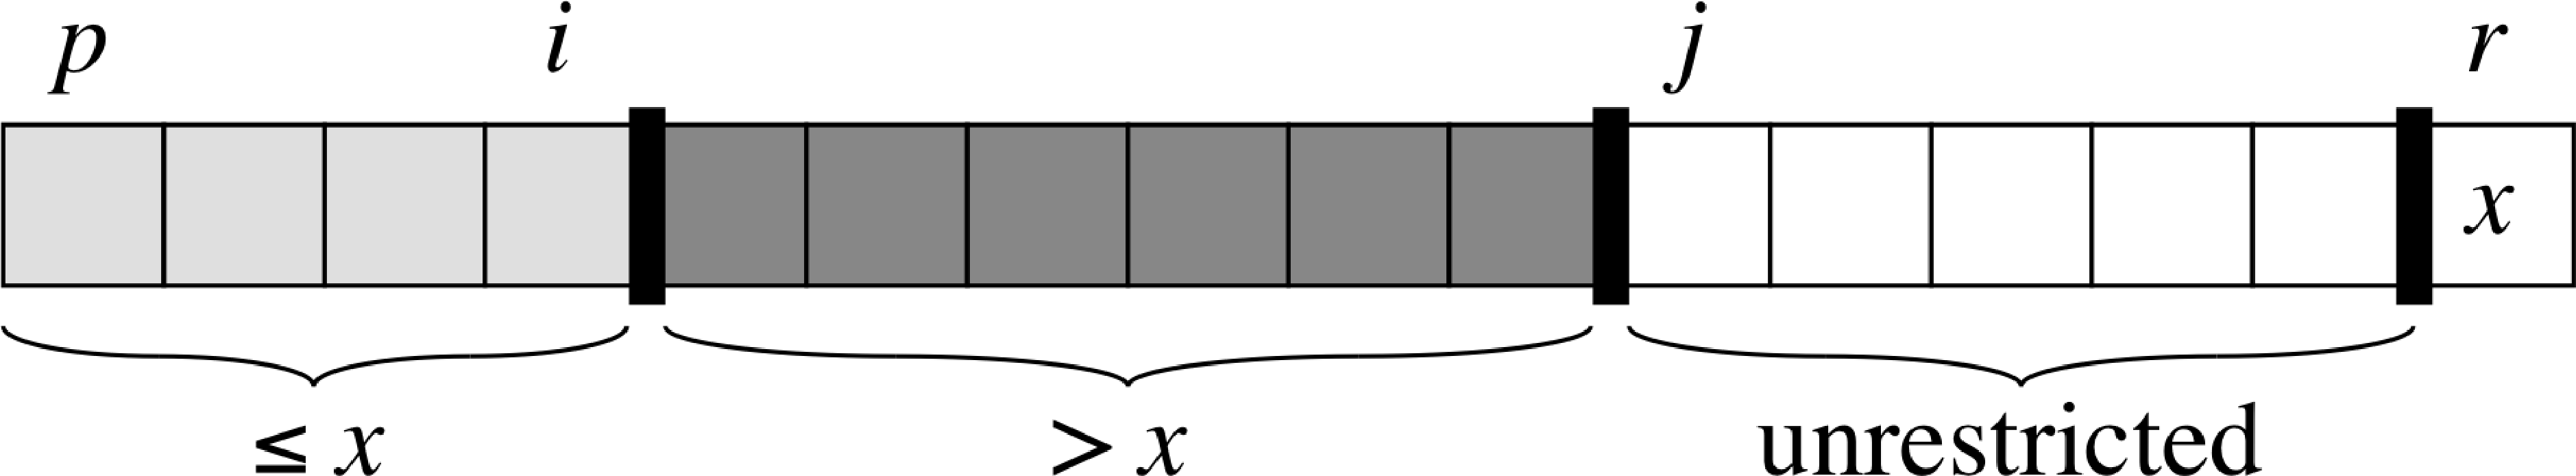
\includegraphics[width=4in]{Fig-7-2.pdf}

\vfill
 Loop invariant:
\begin{enumerate}
  \ii All entries in $A[p,...,i]$ are $\leq$ pivot
  \ii All entries in $A[i+1,...,j-1]$ are $>$ pivot
  \ii $A[r] =$ pivot
\end{enumerate}

\end{frame}

\sect{}
  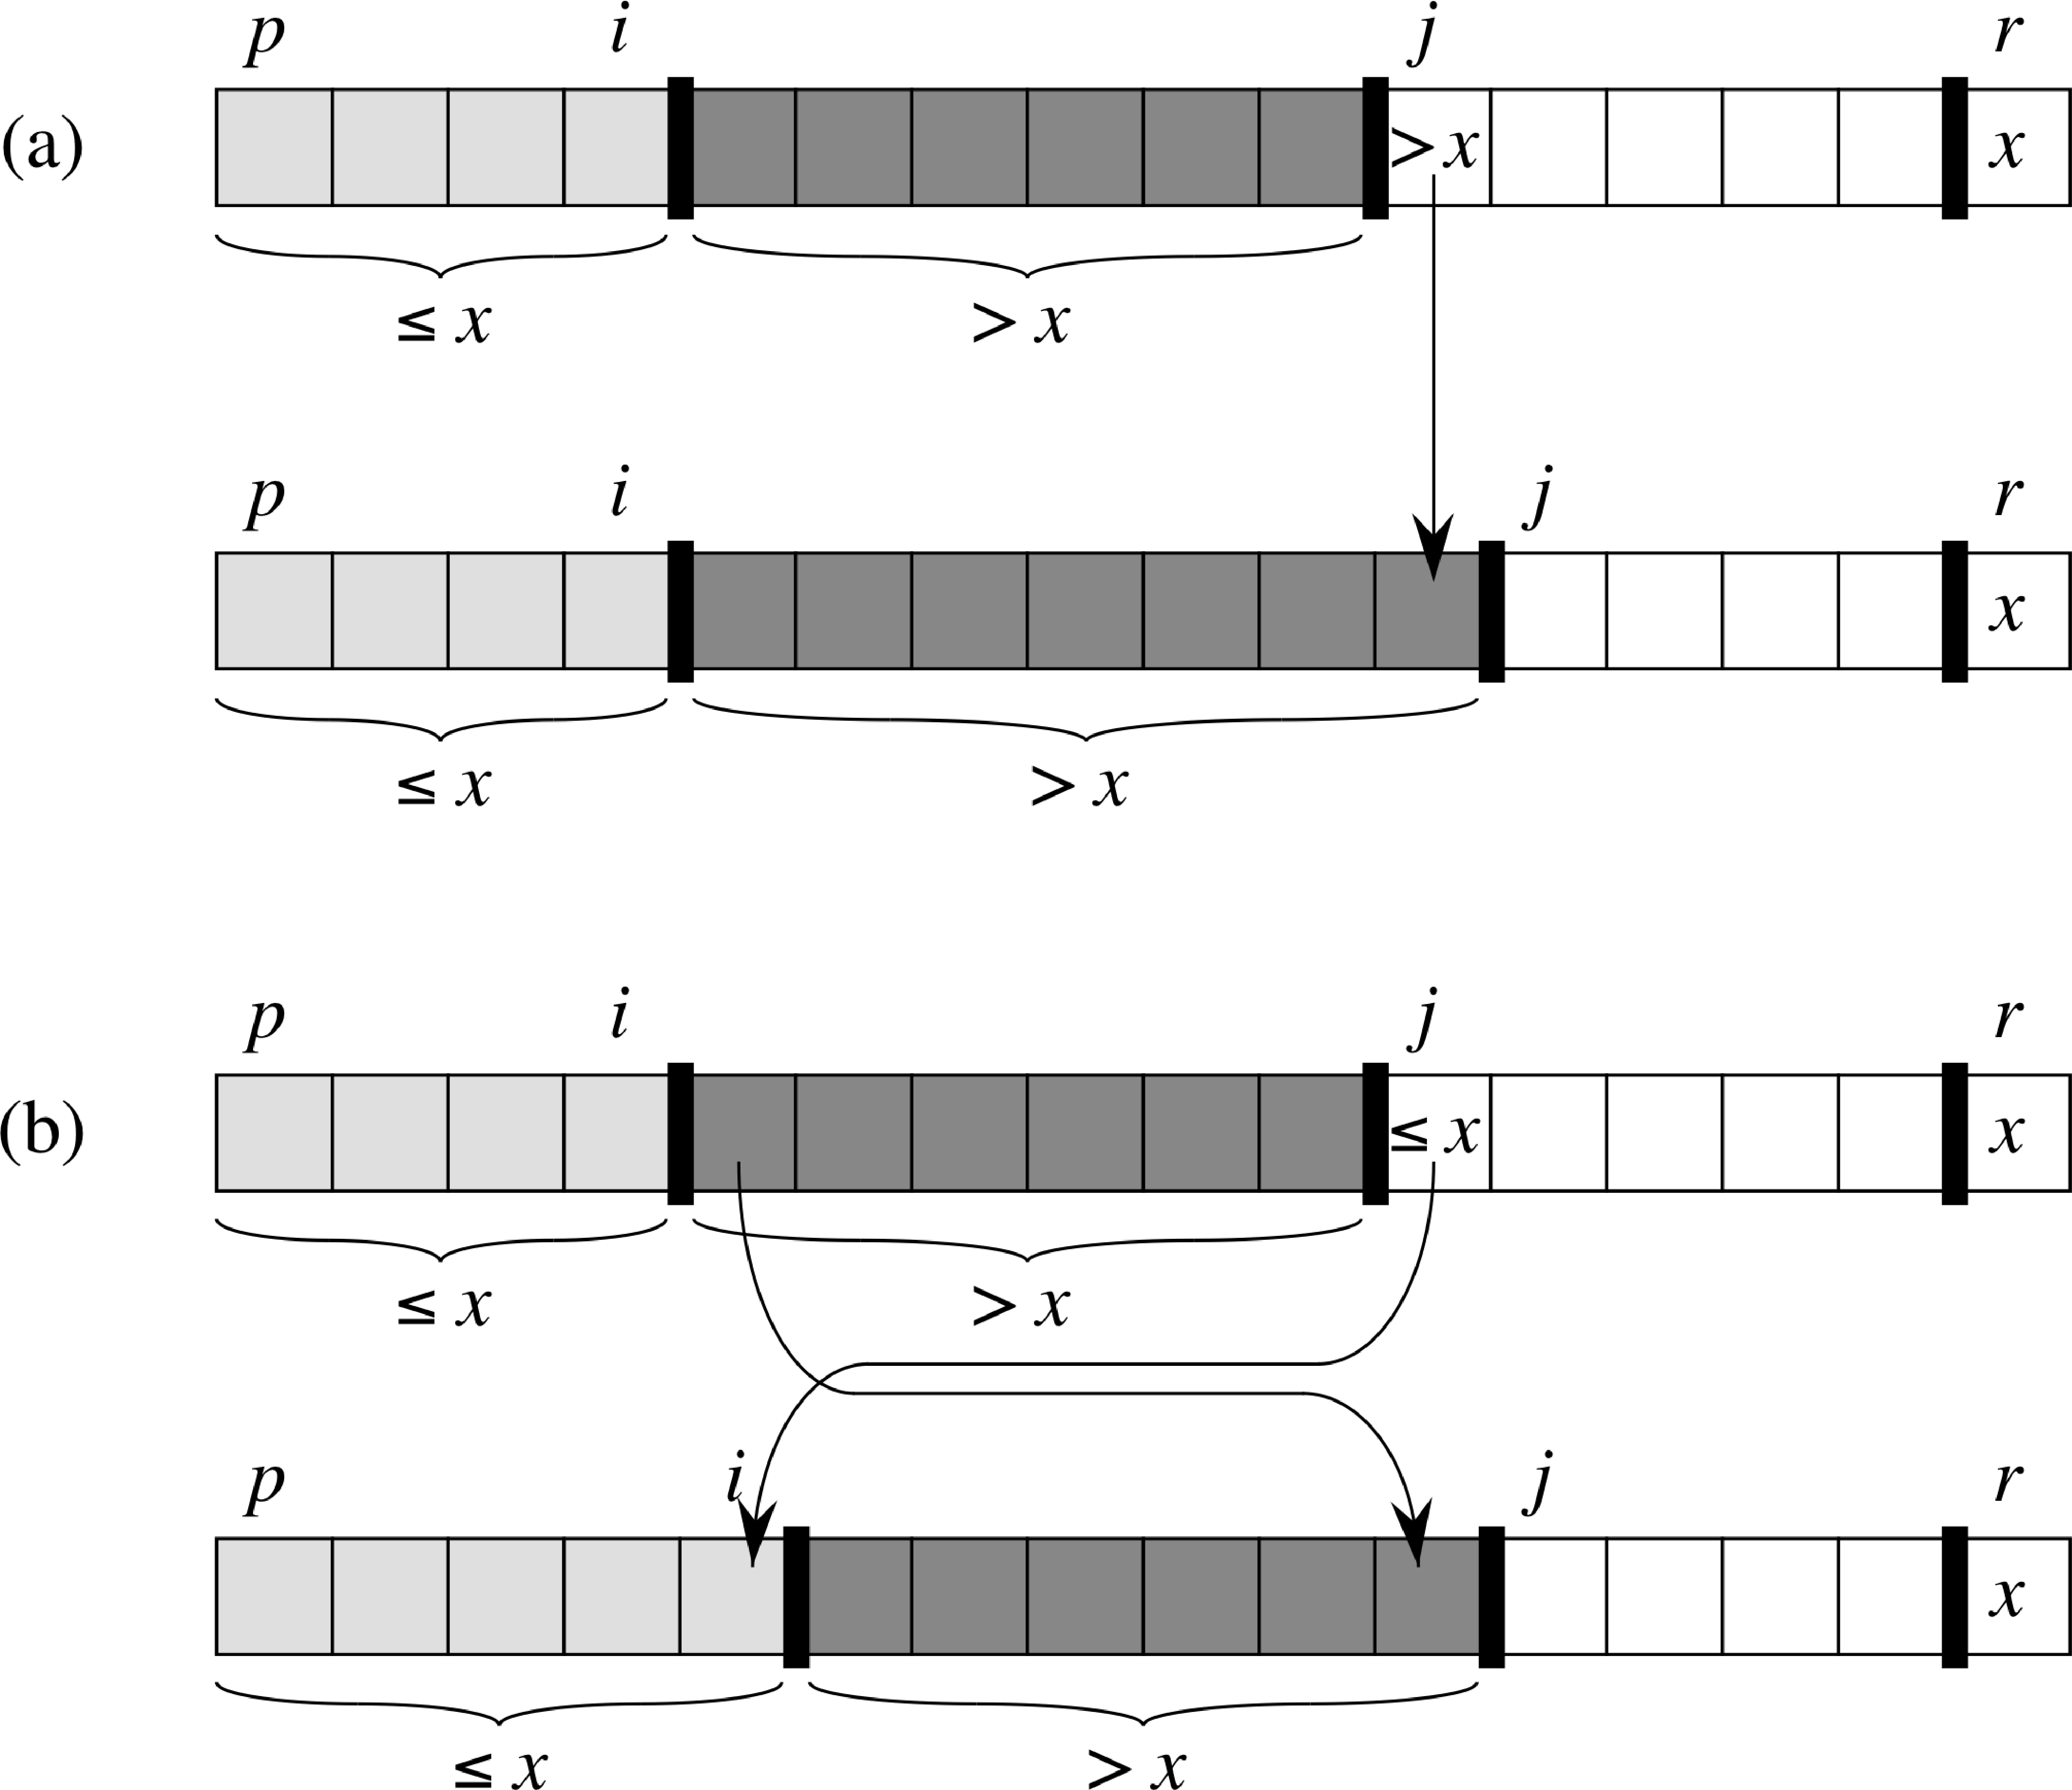
\includegraphics[height=0.9\textheight]{Fig-7-3.pdf}
\end{frame}


\sect{}
\begin{multicols}{2}
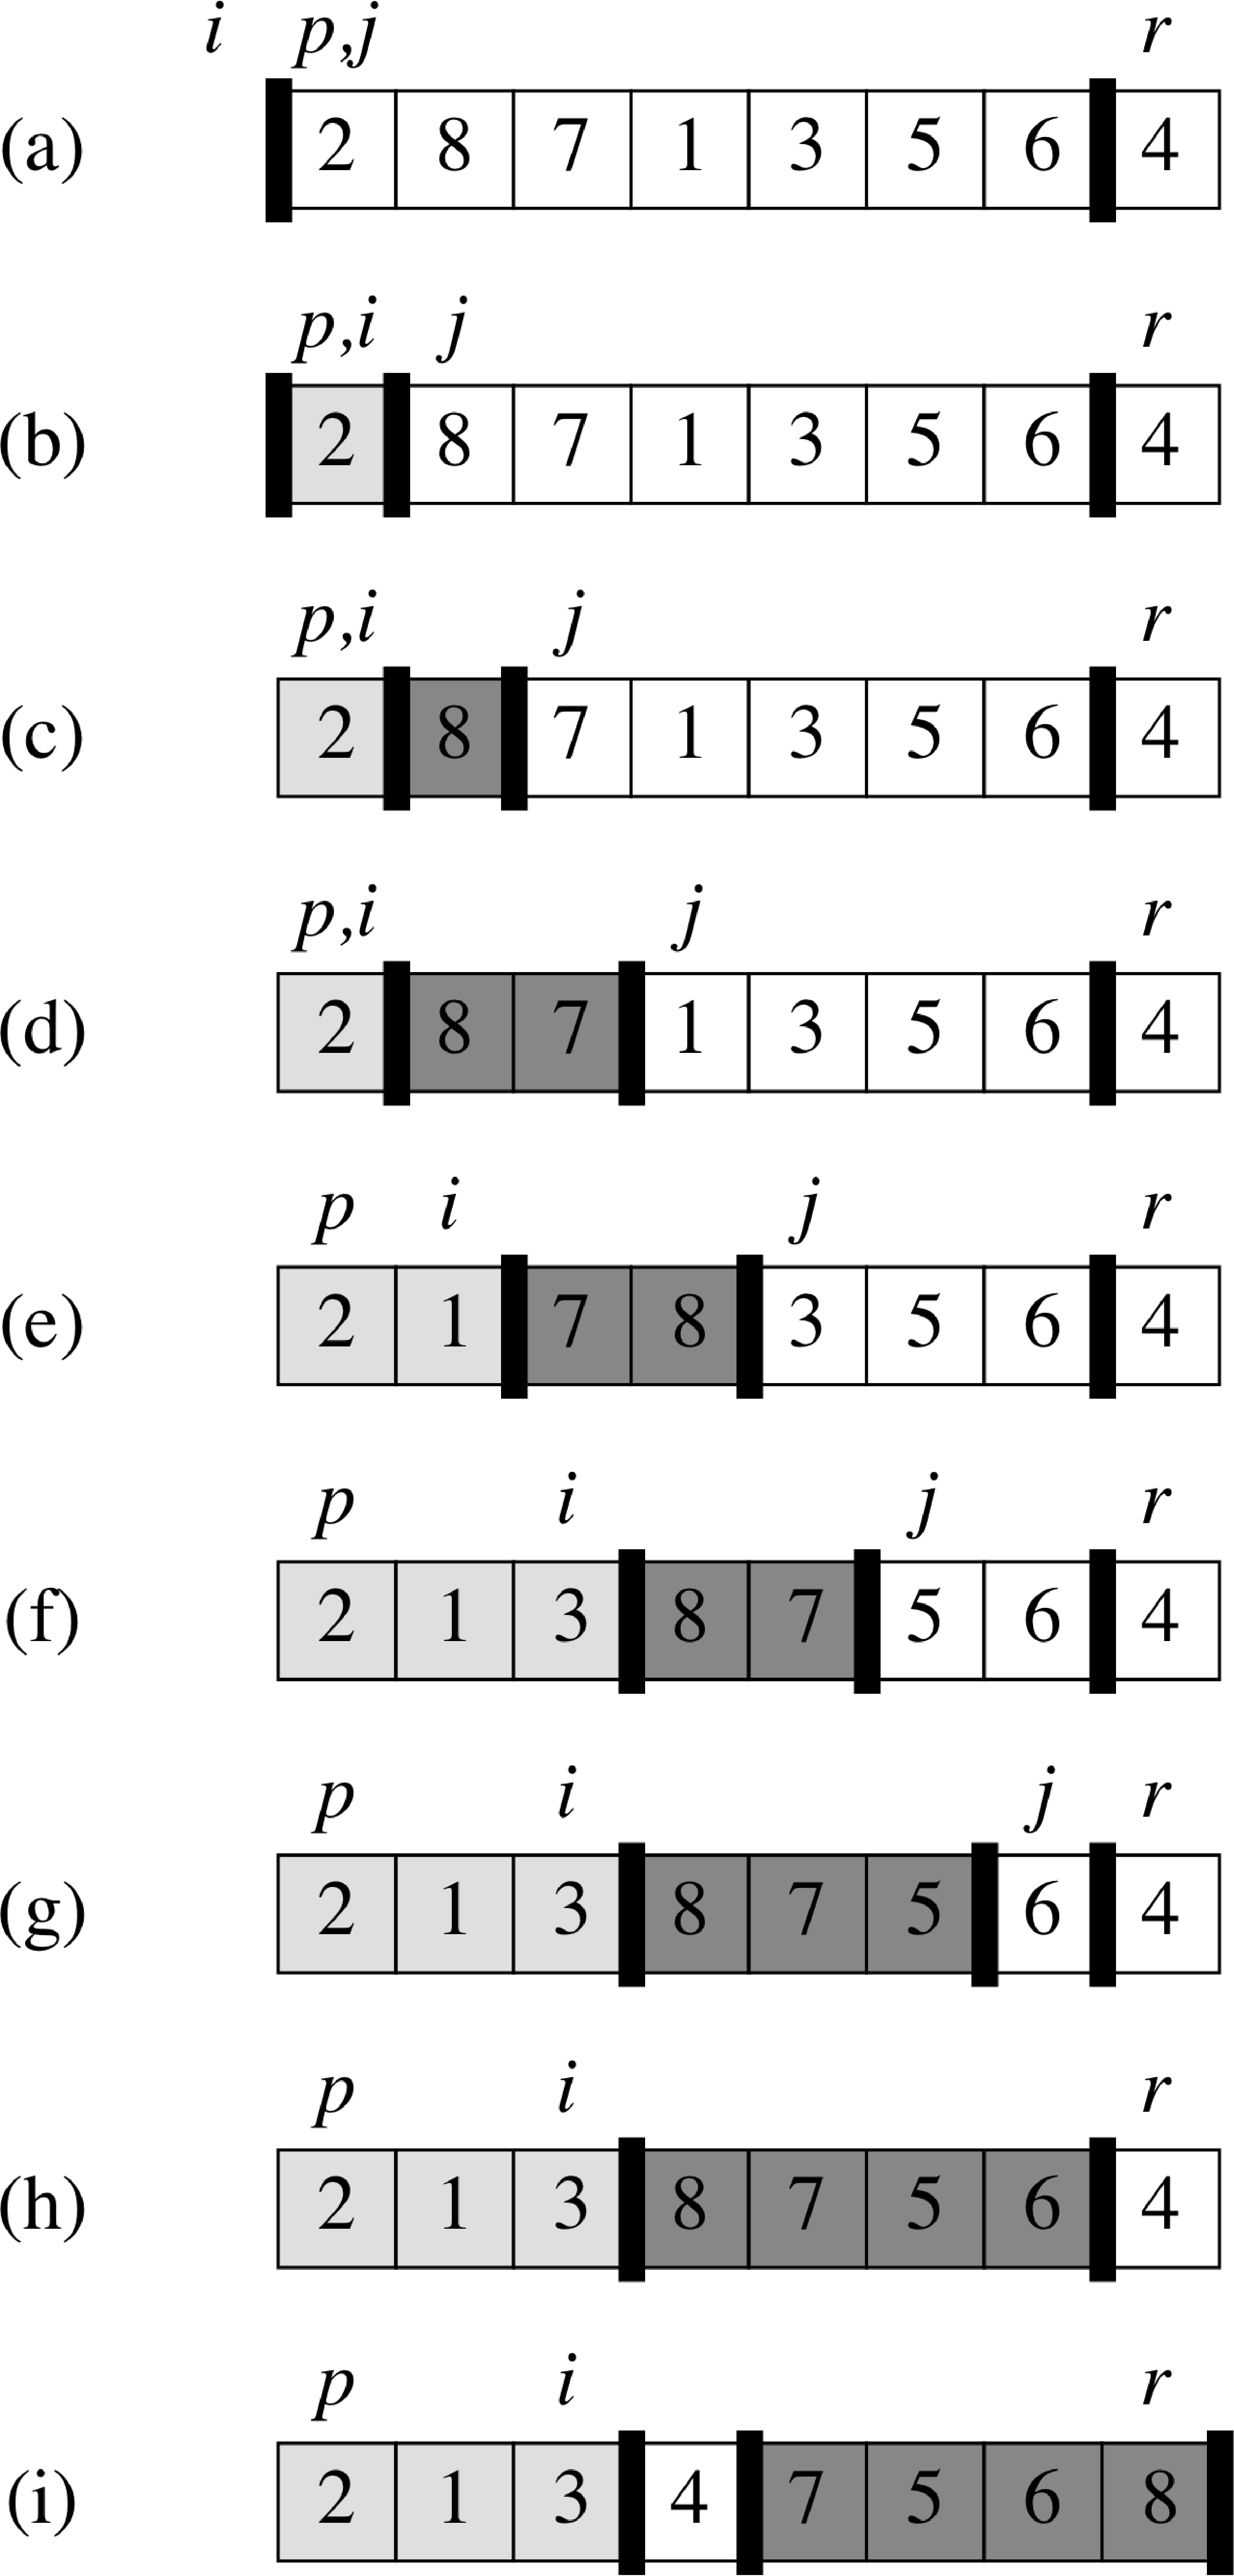
\includegraphics[height=0.9\textheight]{Fig-7-1.pdf}
\columnbreak
\hfill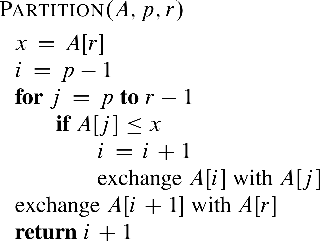
\includegraphics{Partition}
\end{multicols}
\end{frame}

\sect{Partition}

\begin{minipage}{0.6\textwidth}
\begin{codebox}
  \Procname{$\proc{Partition}(A,p,r)$}
  \li $x \gets A[r]$
  \li $i\gets p-1$
  \li \For $j=p$ \To $r-1$ \Do
  \li \If $A[j] \leq x$ \Do
  \li $i \gets i+1$
  \li exchange $A[i]$ with $A[j]$
\End
\End
\li exchange $A[i+1]$ with $A[r]$
\li \Return $i+1$
\end{codebox}
\end{minipage}


\bi
\ii Always selects $A[r]$ as the \textbf{pivot}
\ii Loop invariant:
\begin{enumerate}
  \ii All entries in $A[p,...,i]$ are $\leq$ pivot
  \ii All entries in $A[i+1,...,j-1]$ are $>$ pivot
  \ii $A[r] =$ pivot
\end{enumerate}
\ei

\vfill

$O(n)$


\end{frame}

\sect{Can \textsc{Mergesort} be done in place?}

\resizebox{\linewidth}{!}{
\begin{tabular}{|c|c|c|c|c|c|c|c|c|c|}\hline
  1 & 3 & 5 & 7 & 9 & 0 & 2 & 4 & 6 & 8 \\\hline
  \end{tabular}
}
\vfill
\pause
\bi
\item Yes, but {\em very} tricky!
  \ei
  

\end{frame}

\sect{Running time of quicksort}

\bi
\ii Depends on partitioning of subarrays.
\ii If subarrays are balanced: fast as mergesort.
\ii If subarrays are unbalanced:  slow as insertion sort.
\ei

\end{frame}

\sect{Worst case for quicksort}
\bi
\ii Arrays completely unbalanced.
\ii 0 elements in one and $n-1$ in the other
\ii Recurrence:
\begin{align*}
  T(n) &= T(n-1) + T(0) + \Theta(n)\\
  &= T(n-1) +  \Theta(n)\\
  &= \Theta(n^2)
\end{align*}
\ii Same as insertion sort.
\ii Worst case for quicksort is the array is already sorted.
\ii This is the best case for insertion sort, which is $O(n)$.
\ei

\end{frame}

\sect{Best case for quicksort}
\bi
\ii Each subarray has $n/2$ elements.
\ii Recurrence:
\begin{align*}
  T(n) &= 2T(n/2) + \Theta(n)\\
  &= \Theta(n\lg n)
\end{align*}
\ii Same as mergesort.
\ei


\end{frame}

\sect{``Average'' running time for quicksort}
Assume \textsc{Partition} always makes a 9-to-1 split.
$
  T(n) \leq T(9n/10) + T(n/10) + \Theta(n)
  = O(n\lg n)$

\vfill

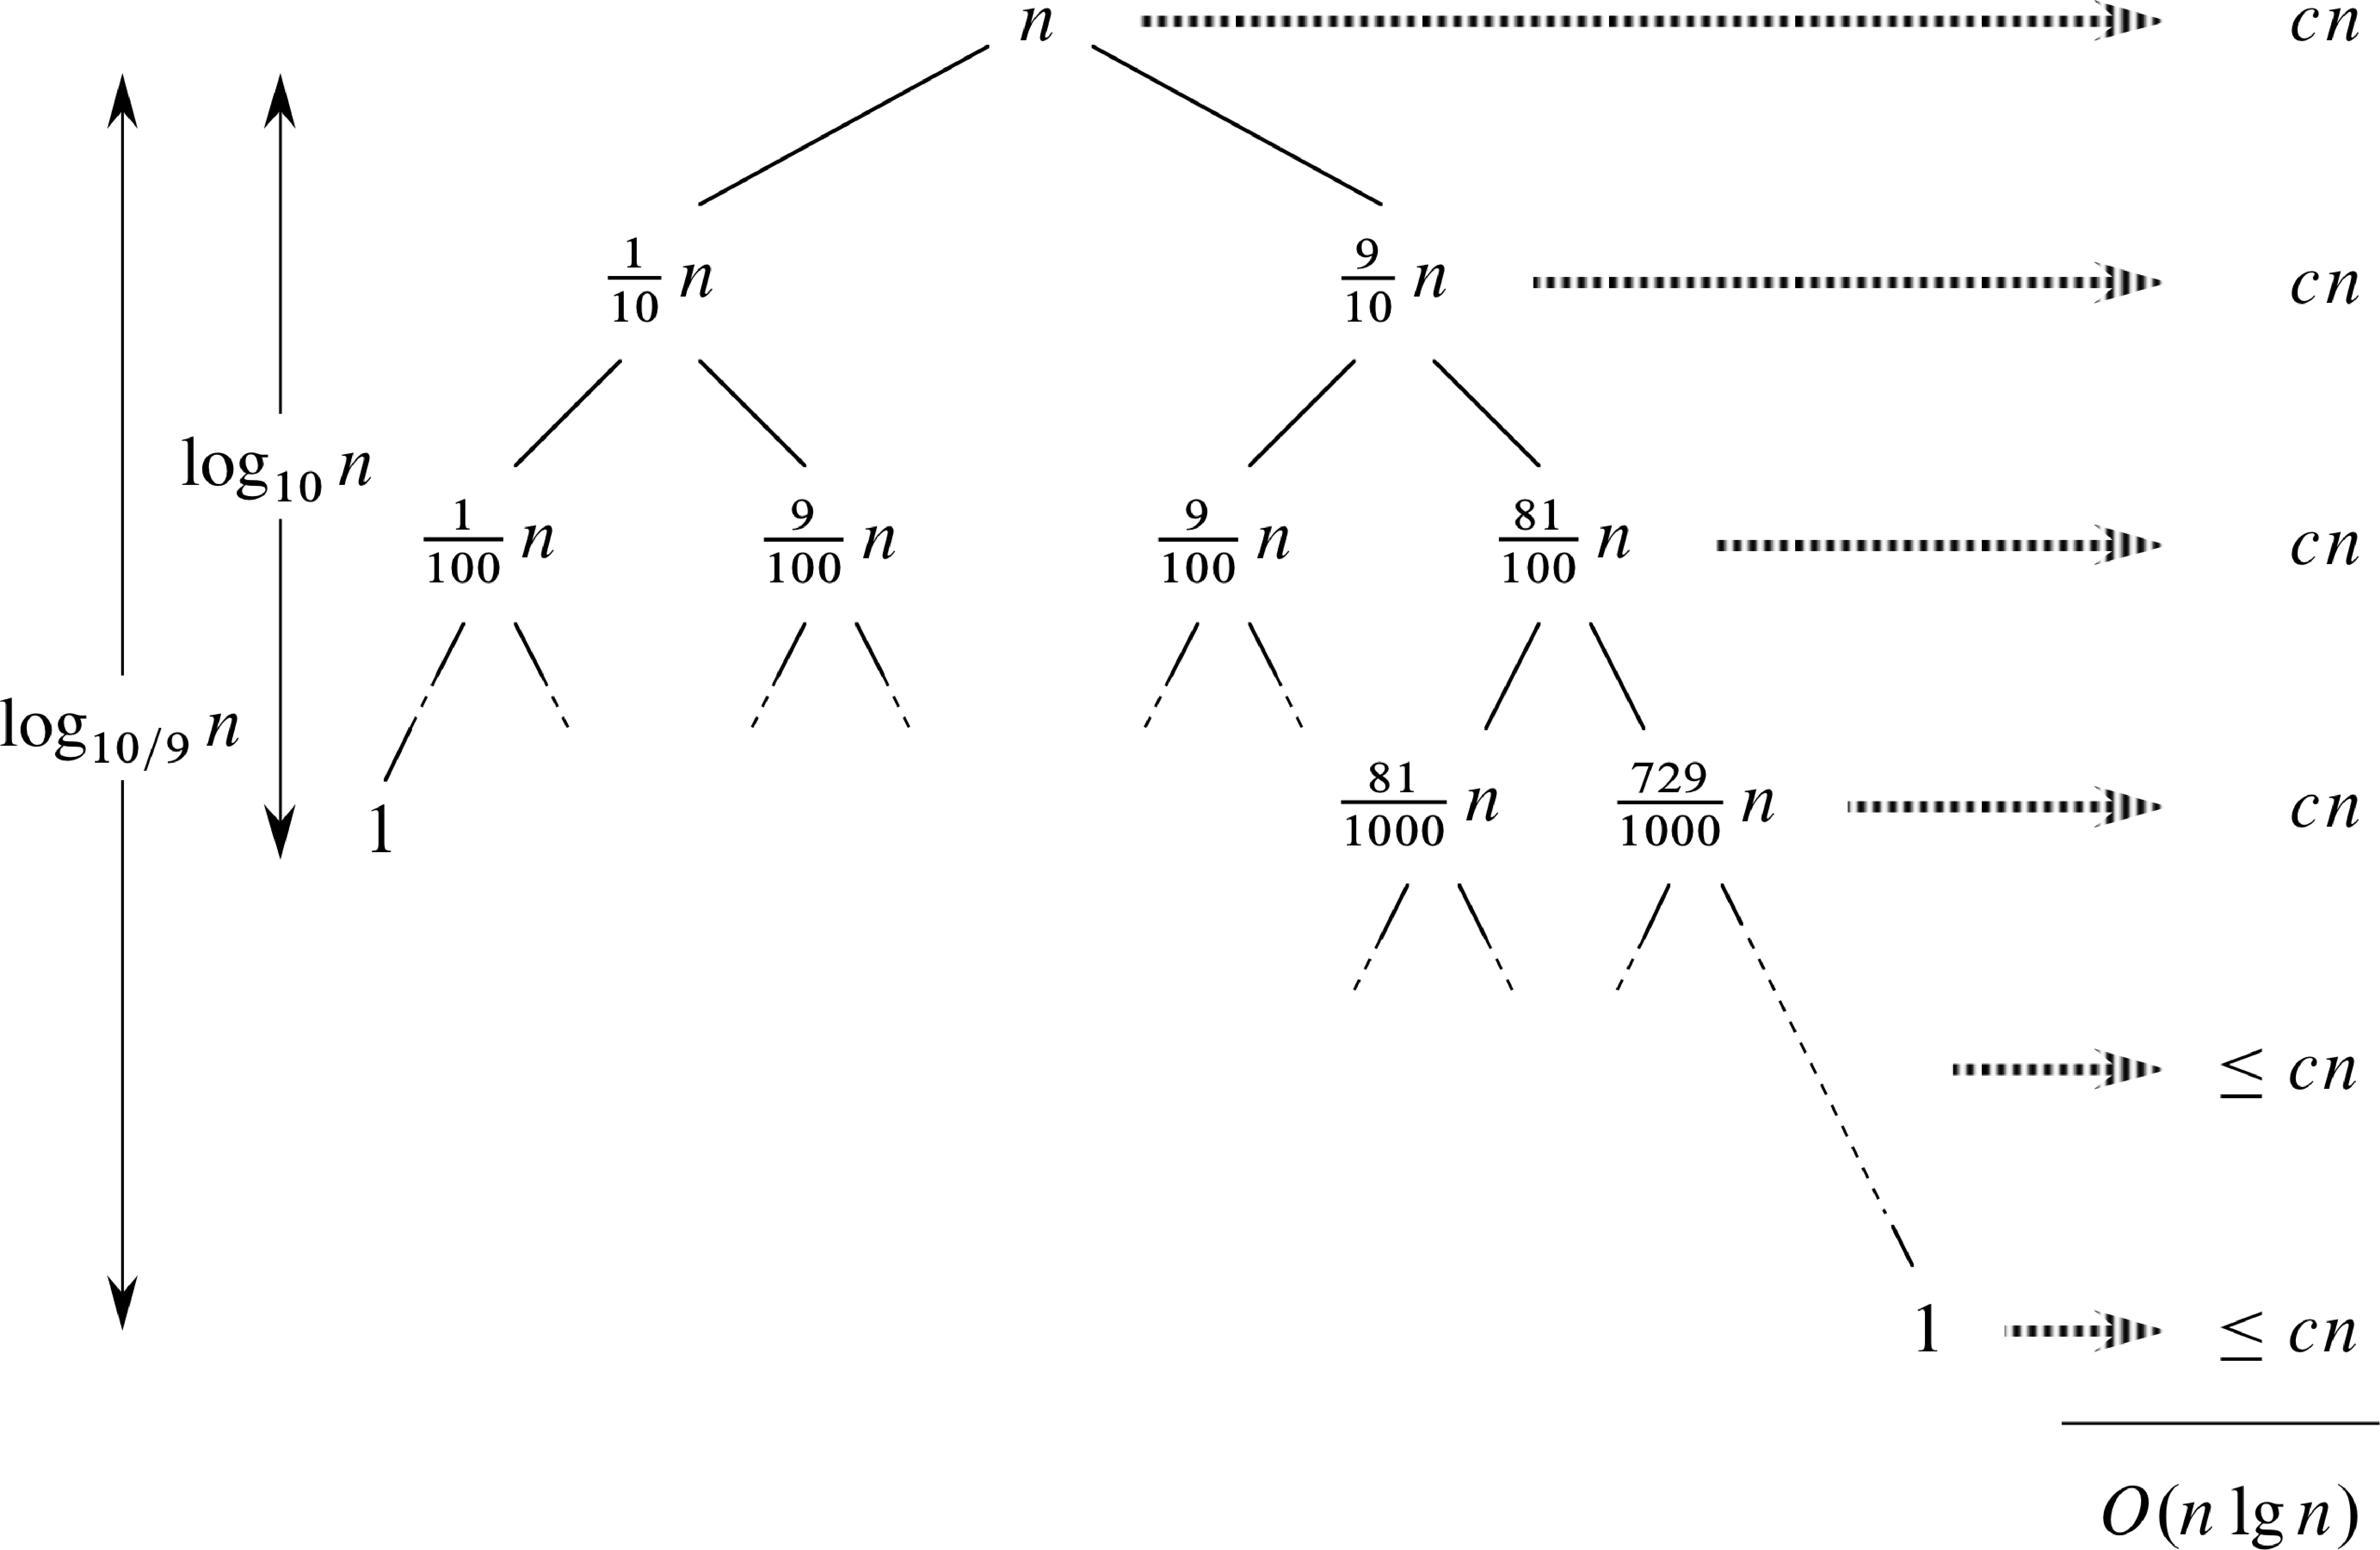
\includegraphics[height=0.75\textheight]{Fig-7-4.pdf}

\end{frame}

\sect{``Average'' running time for quicksort}
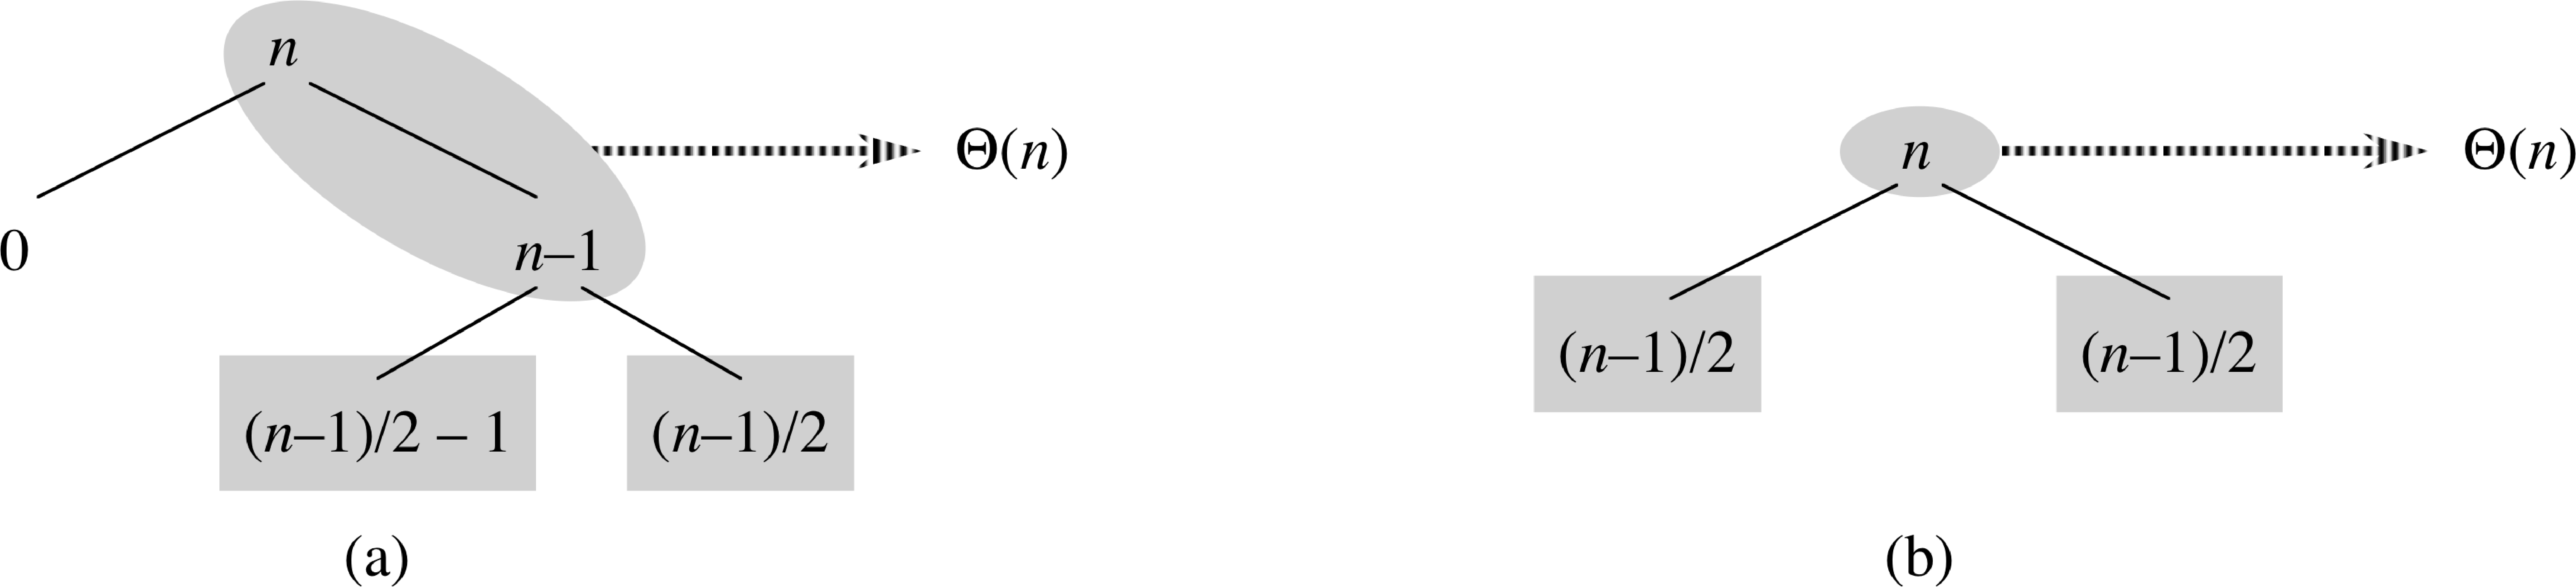
\includegraphics[width=\textwidth]{Fig-7-5.pdf}
\bi
\ii If levels alternate between good and bad splits, still $O(n\lg n)$
\ii If we randomize choice of pivot, what is the probability that
all of the choices will be worst case?
\ii If we randomize choice of pivot, what is the probability that
more than half of the choices will be worst case?
\ei

\end{frame}

\sect{Randomized quicksort}
\bi
\ii Instead of randomizing the entire array, which adds a large
constant factor, just randomize the choice of pivot.
\begin{codebox}
  \Procname{$\proc{Randomized-Partition}(A,p,r)$}
  \li $i \gets \proc{Random}(p,r)$
  \li exchange $A[r]$ with $A[i]$
  \li \Return $\proc{Partition}(a,p,r)$
\end{codebox}
\begin{codebox}
    \Procname{$\proc{Randomized-Quicksort}(A,p,r)$}
  \li \If $p < r$ \Do
  \li $q\gets \proc{Randomized-Partition}(A,p,r)$
  \li $\proc{Randomized-Quicksort}(A,p,q-1)$
  \li $\proc{Randomized-Quicksort}(A,q+1,r)$
\End
\end{codebox}
\ii On average, the splits will be well balanced.
\ii $O(n\lg n)$ virtually guaranteed when $n$ is large.
\ii Stops any bad input from causing worst-case behavior.
\ei

\end{frame}

\sect{Worst-case analysis of randomized quicksort}
\begin{align*}
  T(n) &= \max_{0\leq q\leq n-1} (T(q) + T(n-q-1)) + \Theta(n)
\end{align*}
\bi
\ii \textbf{Guess:} $T(n) \leq cn^2$ for some $c$.
\begin{align*}
  T(n) &\leq \max_{0\leq q\leq n-1} (cq^2 + c(n-q-1)^2) + \Theta(n)\\
  &=c\cdot\max_{0\leq q\leq n-1} (q^2 + (n-q-1)^2) + \Theta(n)
\end{align*}
\ii This is max when $q=0$ or $q=n-1$ (parabolas).
\begin{align*}
  \max_{0\leq q\leq n-1} (q^2 + (n-q-1)^2) \leq (n-1)^2 = n^2 - 2n + 1
\end{align*}
\begin{align*}
  T(n) &\leq cn^2 -c(2n-1) + \Theta(n)\\
  &\leq cn^2 &\mbox{if $c(2n-1)\geq\Theta(n)$}\\
  &= O(n^2)
\end{align*}
\ii Can also show $T(n) =\Omega(n^2)$, so $T(n) =\Theta(n^2)$.
\ei

\end{frame}

\sect{Quicksort}

\begin{codebox}
  \Procname{$\proc{Quicksort}(A,p,r)$}
  \li \If $p < r$ \Do
  \li $q\gets \proc{Partition}(A,p,r)$
  \li $\proc{Quicksort}(A,p,q-1)$
  \li $\proc{Quicksort}(A,q+1,r)$
\End
\end{codebox}

\begin{codebox}
  \Procname{$\proc{Partition}(A,p,r)$}
  \li $x \gets A[r]$
  \li $i\gets p-1$
  \li \For $j=p$ \To $r-1$ \Do
  \li \If $A[j] \leq x$ \Do
  \li $i \gets i+1$
  \li exchange $A[i]$ with $A[j]$
\End
\End
\li exchange $A[i+1]$ with $A[r]$
\li \Return $i+1$
\end{codebox}

\end{frame}

\sect{Average-case analysis of randomized quicksort}
\bi
\ii The dominant cost of the algorithm is in the calls to  \textsc{Partition}. 
\ii \textsc{Partition} removes the pivot from future consideration.
\ii \textsc{Partition} is called at most $n$ times.
\ii Each call to  \textsc{Partition} does a constant amount of work
plus a constant times the number of comparisons done in the \textbf{for}
loop. 
\ii Let $X$ be the total number of comparisons performed in all calls
to  \textsc{Partition}.
\ii Total work done is $O(n+ X)$.
\ii We seek a bound on the total number of comparisons.
\ei

\end{frame}

\sect{Average-case analysis of randomized quicksort}
\bi
\ii Let the elements of $A$ be $z_1,z_2,...,z_n$ with $z_i$ being the
$i$th smallest.
\ii Define $Z_{ij} = \{z_i,z_{i+1},...,z_j\}$
\ii Each pair of elements is compared at most once.
\bi\ii Compared only to the pivot, and then the pivot is removed.\ei
\ii Let $X_{ij} = {I}\{z_i \mbox{ is compared to } z_j\}$
\ii Since each pair is compared at most once,
\begin{align*}
  X &= \sum_{i=1}^{n-1}\sum_{j=i+1}^{n}X_{ij}
\end{align*}


\begin{align*}
  E[X] &= E\left[\sum_{i=1}^{n-1}\sum_{j=i+1}^{n}X_{ij}\right]\\
  &= \sum_{i=1}^{n-1}\sum_{j=i+1}^{n}E[X_{ij}]
  = \sum_{i=1}^{n-1}\sum_{j=i+1}^{n}\pr{z_i \mbox{ is compared to } z_j}
\end{align*}
\ei

\end{frame}

\sect{Probability $z_i$  is compared to  $z_j$ }
\small
\bi
\ii Numbers in separate partitions will not be compared.
\ii If a pivot $x$ is chosen such that $z_i < x < z_j$, $z_i$ and
$z_j$ will not be compared.
\ii If either $z_i$ or $z_j$ is chosen before any other element of
$Z_{ij}$, then it will be compared to every element of $Z_{ij}$,
except itself.
\ii The probability that $z_i$ is compared to $z_j$ is the probability
that either $z_i$ or $z_j$ is chosen first.
\ii There are $j-i+1$ elements of $Z_{ij}$, and pivots are chosen
randomly and independently.
\ii The probability that any one of them is chosen first is
$1/(j-i+1)$.
\ei

\begin{align*}
  \pr{z_i \mbox{ is compared to } z_j}
  &=
  \pr{\mbox{$z_i$ or $z_j$ is chosen first from $Z_{ij}$}}\\
  &=
  \pr{\mbox{$z_i$ is chosen first}} +  \pr{\mbox{$z_j$ is chosen
      first}}  \\
  &=
  \frac{2}{j-i+1}
\end{align*}


\end{frame}

\sect{Expected number of comparisons}

\begin{align*}
  E[X] &=
  \sum_{i=1}^{n-1}\sum_{j=i+1}^{n}\pr{z_i \mbox{ is compared to }
    z_j}\\
&=  \sum_{i=1}^{n-1}\sum_{j=i+1}^{n}  \frac{2}{j-i+1}  \\
  &=  \sum_{i=1}^{n-1}\sum_{k=1}^{n-i}  \frac{2}{k+1}  \\
  &< \sum_{i=1}^{n-1}\sum_{k=1}^{n}  \frac{2}{k}  \\
  &= \sum_{i=1}^{n-1}O(\lg n)\\
  &= O(n\lg n)
\end{align*}

\end{frame}

\end{document}
